\documentclass[11pt,letterpaper]{article}
\usepackage[T1]{fontenc}
\usepackage{lmodern}
\usepackage[margin=1in,headheight=15pt]{geometry}
\usepackage{amsmath,amssymb,amsthm,mathtools}
\usepackage{microtype,graphicx,booktabs,longtable,array}
\usepackage[dvipsnames]{xcolor}
\usepackage{enumitem,fancyhdr,listings}
\usepackage[colorlinks=true,linkcolor=MidnightBlue,urlcolor=MidnightBlue,citecolor=MidnightBlue]{hyperref}
\usepackage[nameinlink,noabbrev]{cleveref}
\definecolor{ink}{HTML}{18364C}
\definecolor{accent}{HTML}{147D92}
\definecolor{light}{HTML}{EEF5F8}
\pagestyle{fancy}
\fancyhf{}
\fancyhead[L]{\small\color{ink}Minkowski's theorem in iPRA}
\fancyhead[R]{\small\color{ink}Finite constructive proof}
\fancyfoot[C]{\thepage}
\setlength{\parskip}{.35em}
\setlength{\parindent}{1.1em}
\setlength{\emergencystretch}{2em}
\setlist{itemsep=.2em,topsep=.3em}
\newtheorem{theorem}{Theorem}[section]
\newtheorem{lemma}[theorem]{Lemma}
\newtheorem{corollary}[theorem]{Corollary}
\newtheorem{proposition}[theorem]{Proposition}
\theoremstyle{definition}
\newtheorem{definition}[theorem]{Definition}
\newtheorem{remark}[theorem]{Remark}
\newcommand{\N}{\mathbb N}
\newcommand{\Z}{\mathbb Z}
\newcommand{\Q}{\mathbb Q}
\newcommand{\R}{\mathbb R}
\newcommand{\ipra}{\mathsf{iPRA}}
\newcommand{\Vol}{\operatorname{vol}}
\newcommand{\Valid}{\operatorname{Valid}}
\newcommand{\Good}{\operatorname{Good}}
\newcommand{\BoxOK}{\operatorname{BoxOK}}
\newcommand{\Inside}{\operatorname{Inside}}
\newcommand{\Sym}{\operatorname{Sym}}
\newcommand{\Mid}{\operatorname{Mid}}
\newcommand{\code}[1]{\texttt{\detokenize{#1}}}
\newcommand{\norminf}[1]{\lVert #1\rVert_\infty}
\newcolumntype{L}[1]{>{\raggedright\arraybackslash}p{#1}}
\lstset{basicstyle=\ttfamily\footnotesize,columns=fullflexible,breaklines=true,
  frame=single,rulecolor=\color{black!15},backgroundcolor=\color{light},
  keepspaces=true,showstringspaces=false}
\begin{document}
\hypersetup{pdftitle={Minkowski's convex-body theorem in intuitionistic primitive recursive arithmetic},
 pdfsubject={A constructive certificate proof and Lean formalization outline},
 pdfkeywords={Minkowski, iPRA, primitive recursive arithmetic, constructive mathematics, Lean}}
\hypersetup{pageanchor=false}
\begin{titlepage}
\vspace*{.45in}
{\color{accent}\sffamily\bfseries RESEARCH NOTE}\par
\vspace{.22in}
{\color{ink}\LARGE\bfseries Minkowski's convex-body theorem\\[.18em]
in intuitionistic primitive\\[.18em] recursive arithmetic\par}
\vspace{.3in}
{\large A finite certificate proof, an explicit rational-polytope\\
construction, and a path to Lean formalization\par}
\vspace{.45in}
Prepared for Vladimir Reshetnikov\\
14 November 2026
\vspace{.5in}
\begin{abstract}
The strict form of Minkowski's theorem admits a direct proof in
intuitionistic primitive recursive arithmetic once its positive volume
premise is expressed by finite inner-volume evidence. Rational boxes in
half the lattice-normalized body are refined to a common mesh. Their
volume forces more cells than residue classes. An explicitly bounded
collision search returns a nonzero integer vector, and symmetry together
with one midpoint puts the associated lattice vector in the body.

We give the complete written proof, a quantifier-free induction audit,
and a quantitative construction of the volume certificate for bounded
rational polytopes. We also prove the exact-threshold theorem for rational
polytopes by an integer-facet dilation argument. For arbitrary represented
real bodies the exact-threshold extension entails LLPO; a rectangle
example isolates that obstruction.

The accompanying exact Python implementation produces and independently
checks witnesses. The Lean sources are an explicitly uncompiled
formalization outline based on the inspected \code{ConciseIPRA} interfaces
in ProveIt. They do not constitute a completed Lean proof or a completed
object-language derivation.
\end{abstract}
\vfill
{\small
Repository snapshot used for the formalization plan:\par
\code{329161f8da0b319d51ba9f6246c4b19d243f7193}\par
Recorded toolchain: \code{leanprover/lean4:v4.32.0}.
}
\end{titlepage}
\pagenumbering{roman}
\hypersetup{pageanchor=true}
{\small\setlength{\parskip}{0pt}\tableofcontents}
\clearpage
\pagenumbering{arabic}
\section{The result and its precise scope}\label{sec:scope}

The theorem requested is the strict convex-body theorem:
if \(n\geq1\), \(L=B\Z^n\) is a full-rank lattice, \(K\subseteq\R^n\)
is convex and symmetric about the origin, and
\begin{equation}\label{eq:classical}
   \Vol(K)>2^n|\det B|,
\end{equation}
then \(K\) contains a nonzero point of \(L\).
The familiar proof uses Blichfeldt's principle on \(K/2\), followed by
symmetry and convexity; see the primary exposition \cite{gorodnik}.
The same geometric last step survives here. We replace the continuous
pigeonhole argument by a finite one whose witness is explicitly computed.

There is a necessary language issue. First-order \(\ipra\) quantifies
over natural numbers. It does not literally quantify over arbitrary
subsets of \(\R^n\), real matrices, or Lebesgue measures. An assertion
that a geometric theorem is \emph{in \(\ipra\)} must specify its arithmetic
representation. The following three results do so.

\begin{enumerate}
\item \textbf{Uniform finite arithmetic theorem.}
There is a fixed primitive recursive extractor for rational box
certificates. Its correctness is provable in \(\ipra\). With a rational
basis and a body given by rational symmetric linear inequalities, both
the input checker and the output checker are fixed primitive recursive
functions, uniformly in the dimension.
\item \textbf{Geometric theorem scheme.}
For each arithmetic formula describing membership of rational
lattice-coordinate points, symmetry, midpoint closure, and a finite
inner-volume witness imply a nonzero integer point. Membership need not
be decidable. The arithmetic extractor does not inspect that formula.
\item \textbf{Rational-polytope theorem.}
For bounded rational symmetric polytopes, the usual finite rational
volume inequality produces the required box certificate with an
explicit primitive recursive mesh bound. The weak inequality
\(\Vol(K)\geq2^n|\det B|\) is also sufficient for these closed rational
polytopes.
\end{enumerate}

For represented real bodies, the strict theorem has the same meaning
when positive volume is supplied as effective inner evidence, or by a
representation with a proved procedure that supplies that evidence.
The exact-threshold theorem for arbitrary real bodies is a different
constructive assertion; \cref{sec:obstruction} proves that it entails
weak sign choice.

\subsection{What is proved and what is implemented}
\begin{center}
\begin{tabular}{p{.48\textwidth}p{.43\textwidth}}
\toprule
Deliverable & Status\\
\midrule
Finite certificate theorem and its iPRA induction audit&
Complete human-readable proof below\\
Quantitative rational-polytope reduction and rational equality case&
Complete written argument, including finite volume lemmas\\
Exact rational extraction and witness validation&
Implemented and exercised on the supplied examples\\
Lean data, targets, and completion plan&
Provided as uncompiled source outlines\\
Final Lean term of type \code{Prf PRAAx [] ...}&
Not supplied; an explicit remaining formalization task\\
\bottomrule
\end{tabular}
\end{center}

These distinctions matter. A correct theorem about Lean's \(\R\) or
\(\N\) does not, merely by being accepted by Lean, establish that
\(\ipra\) proves its arithmetic translation. The final formalization
target must assert object-theory derivability.

\section{The base theory and finite coding}\label{sec:arithmetic}

We use first-order intuitionistic logic with equality. Its nonlogical
language contains \(0,S\), and a function symbol for every finite
primitive recursive definition: zero, successor, projections,
composition, and primitive recursion. There are defining equations for
these symbols, successor separation \(Sx\neq0\), successor injectivity,
and induction
\begin{equation}\label{eq:qfind}
 A(0,\vec p)\ \wedge\
 \forall t\bigl(A(t,\vec p)\to A(St,\vec p)\bigr)
 \ \longrightarrow\ \forall t\,A(t,\vec p)
\end{equation}
only when \(A\) is quantifier-free. All parameters \(\vec p\) are allowed.
This is the presentation explicitly defined by \code{PRAAx} in the
inspected \code{ConciseIPRA/PR.lean} \cite{proveit-pr}; compare also
Moschovakis's discussion of the quantifier-free and first-order
presentations \cite{moschovakis}.

Integers are signed natural-number codes. One possible encoding is
\[
 \iota(z)=
 \begin{cases}2z,&z\geq0,\\-2z-1,&z<0.\end{cases}
\]
A rational is an integer numerator and a positive natural denominator.
Internal numerical calculations may use unreduced pairs and compare
them by cross multiplication. For the formula scheme, however, every
rational argument is in \emph{canonical reduced form}: positive
denominator, coprime numerator and denominator, and \(0=0/1\).
All operations feeding that scheme normalize their results.
Reduction is primitive recursive: compute a gcd by bounded divisor
search and divide exactly. The uniqueness of this normal form follows
from the elementary integer divisibility identities in iPRA.
Finite lists use a fixed canonical sequence coding, so equality of
rational vectors gives equality of their codes.
Malformed codes receive designated default decodings, so every function
is total.

\subsection{Bounded statements are Boolean equations}

It is not legitimate to call a formula quantifier-free merely because
all its quantifiers are bounded. Instead, introduce each finite
arithmetic test \(R(i,\vec p)\) by an explicit primitive recursive
characteristic function, or prove in iPRA that \(R\) is equivalent
to that function equaling \(1\). Denote its bit by \([R(i,\vec p)]\).
Then
\[
 \forall i<t\,R(i,\vec p)
 \quad\hbox{is represented by}\quad
 \prod_{i<t}[R(i,\vec p)]=1.
\]
Bounded existentials use finite maxima or a bounded first-witness
function. A finite conjunction of equations and inequalities is likewise
a Boolean equation. All inductions used below are on such equations or
quantifier-free combinations of them.

Natural equality, order, and their finite Boolean combinations are
decidable in this theory. Using a case split on a computed bit therefore
does not introduce unrestricted excluded middle. In particular, a
failed bounded search can be ruled out by arithmetic contradiction,
leaving its successful Boolean branch and its stored witness.

\subsection{The meaning of primitive recursive uniformity}

Our uniform algorithm takes \emph{finite numerical data}: dimensions,
matrices, rational endpoints, and finite lists. No total primitive
recursive interpreter for arbitrary primitive recursive programs is
assumed. Such an interpreter is unavailable. When an application uses
primitive recursive real approximation functions, those functions are
fixed in advance, or their finite computations are supplied as bounded
traces checked by a fixed verifier.

This distinction also prevents a false inference from eventual
termination to availability in \(\ipra\).
Every search in the main theorem has a displayed bound obtained from
its finite input.

\section{Finite inner-volume certificates}\label{sec:certificate}

First work in lattice coordinates. Write
\[
 P=B^{-1}K,\qquad D=\tfrac12P.
\]
Convexity and symmetry are preserved by this linear change of
coordinates, and the desired output is \(z\in\Z^n\setminus\{0\}\)
with \(z\in P\). Its physical lattice vector is \(Bz\).

\begin{definition}[A box certificate]\label{def:cert}
A finite inner-volume certificate for \(D\) is a nonempty finite list
of rational boxes
\[
 Q_j=\prod_{k=0}^{n-1}[\ell_{jk},u_{jk}]
 \quad(0\leq j<s)
\]
such that:
\begin{enumerate}
\item every side length is positive;
\item the interiors of distinct boxes are disjoint;
\item every box is contained in \(D\);
\item their total rational content satisfies
\begin{equation}\label{eq:box-volume}
 W:=\sum_{j<s}\prod_{k<n}(u_{jk}-\ell_{jk})>1.
\end{equation}
\end{enumerate}
\end{definition}

Here containment can mean containment of all rational points; that is
all the arithmetic proof will use. When the boxes are genuinely
contained in a real body, this rational containment follows immediately.
Interiors may be disjoint while boundaries touch. A cell center will be
used so that no choice on a shared boundary is needed.

The certificate gives positive volumetric evidence, not a lattice point:
it consists only of rational endpoints and inclusion facts.
It need not enumerate all points in the body, decide the body's
boundary, or supply the eventual collision.

\subsection{A pure arithmetic checker and a membership scheme}

Let \(\BoxOK(n,c)\) check the numerical parts of
\cref{def:cert}: correct rational codes, positive sides, disjoint
interiors, and \(W>1\). Disjointness is decidable by
\begin{equation}\label{eq:box-disjoint}
 \forall i<j<s\ \exists k<n\
 \bigl(u_{ik}\leq\ell_{jk}\ \vee\
       u_{jk}\leq\ell_{ik}\bigr).
\end{equation}
Every quantifier here is a finite loop compiled into a bit.

Let \(\Phi(q)\) be any fixed arithmetic formula on canonically coded rational
\(n\)-vectors. Additional numerical parameters are suppressed.
Write \(\widehat z\) for the canonical rational embedding of a coded
integer vector \(z\).
Define
\begin{align*}
 \Sym_\Phi&:\quad
   \forall q\,(\Phi(q)\to\Phi(-q)),\\
 \Mid_\Phi&:\quad
   \forall q,r\,\bigl(\Phi(q)\wedge\Phi(r)
       \to\Phi((q+r)/2)\bigr),\\
 \Inside_\Phi(c)&:\quad
   \forall j<s\ \forall q\in Q_j\ \Phi(2q).
\end{align*}
The usual well-formed vector guards are implicit in these displayed
abbreviations and are explicit in a coded version. The interpretation
is \(\Phi(q)\equiv Bq\in K\).

\begin{theorem}[Certificate form of Minkowski in iPRA]\label{thm:main}
There is a fixed primitive recursive function \(F\) such that, for every
formula \(\Phi\) as above, \(\ipra\) proves
\[
\begin{split}
 n\geq1\ \wedge\ \BoxOK(n,c)\ \wedge\
 \Inside_\Phi(c)\ \wedge\ \Sym_\Phi\ \wedge\ \Mid_\Phi\\
 \longrightarrow\
 \bigl(F(n,c)\in\Z^n\ \wedge\ F(n,c)\neq0\
      \wedge\Phi(\widehat{F(n,c)})\bigr).
\end{split}
\]
The output can include an index of a nonzero coordinate and the two
cell indices that justify membership. No induction on \(\Phi\) is used.
Canonical rational operations are essential here: arbitrary formulas
on unreduced fraction codes need not respect equality of rational values.
\end{theorem}

When \(B\) is rational and
\begin{equation}\label{eq:slab}
 K=\{x:\ |a_j\cdot x|\leq b_j\quad(j<t)\}
\end{equation}
has rational rows and bounds, all certificate conditions, including
containment, have one fixed primitive recursive checker.
For a row \(a_j\), put \(\alpha=2a_jB\). Its range on a box is exactly
the interval with endpoints
\[
 \sum_k\min(\alpha_k\ell_k,\alpha_k u_k),
 \qquad
 \sum_k\max(\alpha_k\ell_k,\alpha_k u_k).
\]
Checking that this interval lies in \([-b_j,b_j]\) proves containment.
This yields a single uniform theorem about coded rational data,
as well as the abstract formula scheme.

\section{Complete proof of the certificate theorem}\label{sec:proof}

\subsection{Refine the boxes to an integer grid}

Choose a positive common multiple \(m\) of every endpoint denominator.
The least common multiple is convenient; their product is a simpler
primitive recursive upper bound. Set
\[
 L_{jk}=m\ell_{jk}\in\Z,\qquad U_{jk}=mu_{jk}\in\Z.
\]
For each box enumerate
\[
 A_j=\{a\in\Z^n:\ L_{jk}\leq a_k<U_{jk}\ \ (k<n)\}.
\]
The vector \(a\) identifies a grid cell and its center:
\[
 C_a=\prod_{k<n}[a_k/m,(a_k+1)/m],
 \qquad c_a=\frac{a+\tfrac12\mathbf1}{m}.
\]
If \(a\in A_j\), then \(C_a\subseteq Q_j\) and \(c_a\) lies
strictly inside every coordinate interval of \(Q_j\).

The sets \(A_j\) are pairwise disjoint. If \(a\) belonged to two,
then \(c_a\) would be in both box interiors, contrary to
\cref{eq:box-disjoint}. Thus the concatenated enumeration has no
repeated integer vector. Its length is
\begin{equation}\label{eq:cell-count}
 N=\sum_{j<s}\prod_{k<n}(U_{jk}-L_{jk})
   =m^n\sum_{j<s}\prod_{k<n}(u_{jk}-\ell_{jk})
   =m^nW>m^n.
\end{equation}
This is an exact rational identity. It is not an asymptotic lattice
count, and no error estimate is being suppressed.

The enumeration needs no search over an unbounded region. A box
with widths \(d_k=U_k-L_k\) has \(\prod_kd_k\) positions.
Decode each local index by successive quotient and remainder
operations with these positive radices. Choose its box by the
finite list of cumulative counts. This gives a primitive recursive
random-access enumeration of all \(N\) cells. Only its first
\[
                    H+1,\qquad H=m^n,
\]
entries are needed.

\subsection{Finite pigeonhole with an explicit witness}

\begin{lemma}[Bounded color collision]\label{lem:php}
Given a finite sequence \(d_0,\ldots,d_H\) with \(0\leq d_i<H\)
and \(H\geq1\), a bounded primitive recursive search returns
\(i<j\leq H\) with \(d_i=d_j\). Its correctness is provable using
quantifier-free induction.
\end{lemma}

\begin{proof}
Search all \(\binom{H+1}{2}\) pairs \(i<j\), recording the first
equality. Here is a counting proof that the failure bit of this
bounded search cannot equal \(1\).

For \(r<H\) and \(t\leq H+1\) define
\[
                   c_r(t)=\sum_{i<t}[d_i=r].
\]
Finite summation and the fact that each \(d_i\) has exactly one
value in \(\{0,\ldots,H-1\}\) give
\begin{equation}\label{eq:count-conserve}
                     \sum_{r<H}c_r(t)=t.
\end{equation}
Verify this by induction on \(t\): at the next step precisely
the summand with \(r=d_t\) increases by \(1\).
The assertion about all other summands is bounded and Boolean,
so the induction invariant is quantifier-free after the
definitions in \cref{sec:arithmetic}.

If no equal pair occurs in the first \(t\) positions, then
\(c_r(t)\leq1\) for every \(r<H\). Constructively, scan the
positions with a one-bit flag recording whether \(r\) has
already appeared: a second occurrence gives an explicit
equal pair. The scan invariant is again a bounded Boolean
equation. It follows that
\[
                    t=\sum_{r<H}c_r(t)\leq H.
\]
At \(t=H+1\) this is impossible. The search result is a
decidable Boolean, so its successful branch holds with its
stored indices. This uses no inference from a bare double
negation of an unbounded existential statement.
\end{proof}

A table of previously encountered colors implements the same proof
more efficiently: the first repeat returns a pair, and without
a repeat each input increases occupied slots by one.
The reference code uses this table; the Lean outline starts with
the simpler bounded pair search. Both realize the same finite
theorem.

\subsection{Color by residues and divide the exact difference}

For an integer vector \(a\), let \(r_k(a)\) be its Euclidean
remainder modulo \(m\), including when \(a_k\) is negative:
\[
             a_k=mq_k(a)+r_k(a),\qquad 0\leq r_k(a)<m.
\]
Encode the residue vector by a single color
\[
                 \rho_m(a)=\sum_{k=0}^{n-1}r_k(a)m^k.
\]
Then \(0\leq\rho_m(a)<m^n=H\).
Equal colors have equal coordinate remainders: for \(m\geq2\),
repeatedly take remainder and quotient modulo \(m\); for \(m=1\),
every remainder is \(0\), so the assertion is immediate.

Apply \cref{lem:php} to the first \(H+1\) cell indices.
There are distinct \(a,b\) with identical remainders.
Define
\begin{equation}\label{eq:z}
                z_k=q_k(a)-q_k(b)=\frac{a_k-b_k}{m}\in\Z.
\end{equation}
This is exact division, not rounding. If every \(z_k\) were
zero, then \(a=b\), a contradiction. Since the vector is
finite, a scan finds an actual coordinate \(k<n\) with
\(z_k\neq0\).

\subsection{Use symmetry and a single midpoint}

The certificate gives \(\Phi(2c_a)\) and \(\Phi(2c_b)\).
Symmetry gives \(\Phi(-2c_b)\), and midpoint closure gives
\[
                  \Phi\!\left(\frac{2c_a+(-2c_b)}2\right).
\]
The common half-cell offset cancels:
\begin{equation}\label{eq:center-cancel}
 \frac{2c_a-2c_b}{2}
 =c_a-c_b
 =\frac{a+\frac12\mathbf1-b-\frac12\mathbf1}{m}
 =z.
\end{equation}
Both sides are normalized to the canonical rational-vector code, so
this equality is also equality of numerical codes. Equality replacement
therefore gives \(\Phi(\widehat z)\), proving \cref{thm:main}.

In physical coordinates put \(v=Bz\). It is a lattice vector
by definition. If \(B\) is injective, \(z\neq0\) implies
\(v\neq0\). The same calculation reads
\[
                      v=\frac{2Bc_a+(-2Bc_b)}2\in K.
\]
For rational \(B\), the condition \(\det B\neq0\) supplies
injectivity by the adjugate identity or exact Gaussian
elimination. For a represented real basis, injectivity
must be part of its constructive full-rank data; see
\cref{sec:real}.

\begin{figure}[htbp]
\centering
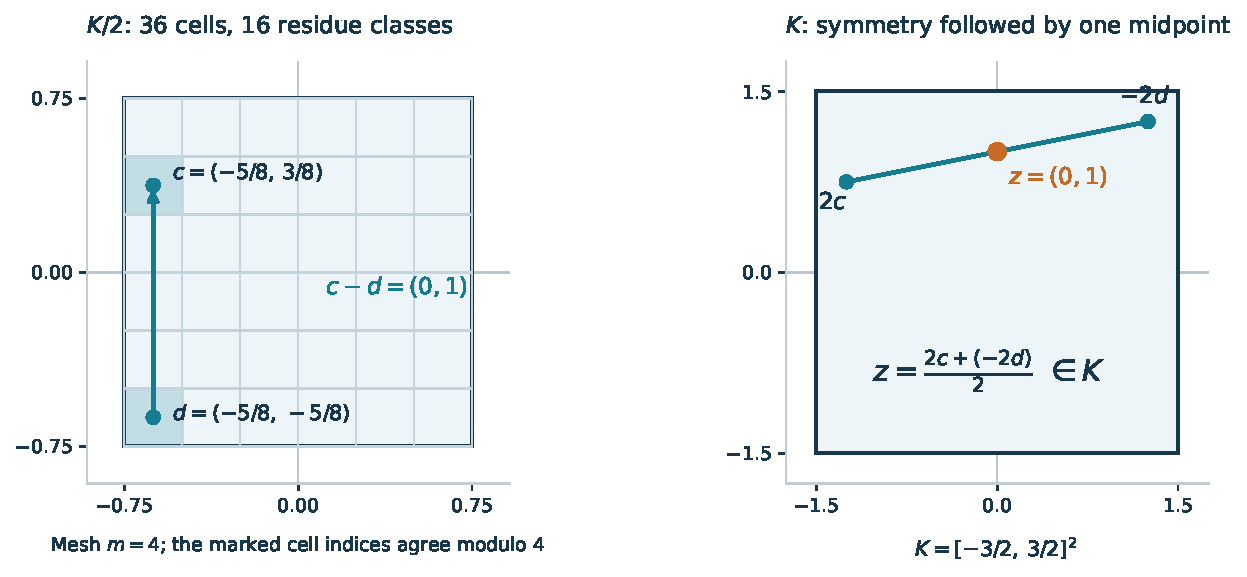
\includegraphics[width=\textwidth]{finite_minkowski.pdf}
\caption{The exact square example. The two selected normalized
centers have an integer difference. Doubling, reflecting one point,
and taking the midpoint places that difference in the original body.}
\label{fig:example}
\end{figure}

\section{Why this is an iPRA proof}\label{sec:audit}

The argument separates arithmetic induction from geometric
membership. This section records the precise audit needed for
the proof-theoretic claim.

\subsection{A fixed correctness equation}

For the rational matrix and slab format, let \(c\) code the
complete finite input. Define fixed primitive recursive functions
\[
                          V(c),\qquad E(c),\qquad G(c,w)
\]
for validation, extraction, and output checking. Invalid
input receives a default output. The uniform arithmetic
theorem is
\begin{equation}\label{eq:object}
 \ipra\vdash\forall c\bigl(V(c)=1\to G(c,E(c))=1\bigr).
\end{equation}
Here \(G\) checks a nonzero integer coefficient vector, its
two contributing cell indices, the scaled-difference
identities, and membership of the returned rational
lattice vector. The witness includes enough data to
verify these claims directly.

For the abstract \(\Phi\) scheme, first prove the purely
arithmetic cell theorem without \(\Phi\). Then instantiate
the two box containment premises and apply symmetry and
midpoint closure once. There is no induction on an
arbitrary body-membership formula and no decision procedure
for it.

\subsection{All required inductions}

\begin{longtable}{L{.25\textwidth}L{.65\textwidth}}
\toprule
Part of the argument & Quantifier-free invariant or identity\\
\midrule
\endhead
Signed quotient/remainder&
\(a=mq+r\) with \(0\leq r<m\), encoded by integer-code equations\\
Mixed-radix enumeration&
Current digits reconstruct the index; digits stay within
their finite coordinate ranges\\
Cell counting&
Prefix count equals the finite sum of products of side widths\\
Disjoint enumeration&
The bounded pairwise-inequality bit is \(1\); a repeated
cell center violates the separating-coordinate check\\
Residue coding&
Partial color equals the partial base-\(m\) sum and is
below \(m^k\); equality is decoded by quotient/remainder\\
Finite pigeonhole&
\(\sum_{r<H}c_r(t)=t\), and the no-repeat bit implies
\(\prod_{r<H}[c_r(t)\leq1]=1\)\\
Nonzero output&
A bounded first-nonzero-coordinate scan; failure means
equality of the two coded vectors\\
Matrix and slab arithmetic&
Finite distributivity and rational cross-multiplication identities\\
\bottomrule
\end{longtable}

These assertions concern finite arrays or explicitly
constructed integers. Every bound in a displayed bounded
quantifier is a primitive recursive term. Replacing that
quantifier by a Boolean fold gives a legitimate induction
instance of \cref{eq:qfind}.

Rational algebra is finite signed-integer algebra with
positive denominators. A displayed division by \(m\) is
justified by \(m\geq1\); a rational inequality can be
multiplied by its positive denominator. The identity
\cref{eq:cell-count} needs only finite products, finite
sums, and distributivity. The geometric last step uses
equality replacement, implication elimination, and
conjunction; it has no inductive content.

\subsection{Explicit bounds}

Let \(D_0\) be the product of all endpoint denominators.
We may use \(m=D_0\), or compute a smaller common multiple.
For a valid certificate,
\begin{align*}
 &m\leq D_0,\qquad H=m^n,\\
 &\text{cells required by the extractor}\leq H+1,\\
 &\text{pairs in a direct collision search}\leq H(H+1)/2,\\
 &\text{color-table slots}=H.
\end{align*}
Each cell is decoded with at most \(s\) prefix comparisons
and \(n\) mixed-radix operations. If every box lies in
\([-R,R]^n\), then its centers do too, so
\begin{equation}\label{eq:coefficient-bound}
                              \norminf{z}\leq2R.
\end{equation}

The sequence encodings have primitive recursive bounds as
well. An array of length \(L\) whose entries are below \(M\)
can be encoded in base \(M+1\) below \((M+1)^L\), together
with its length and base. Signed coordinates and rational
pairs admit the same kind of bound after their components
are bounded. Bounded iteration of a coded state is ordinary
primitive recursion. No claim here is polynomial-time:
the purpose is the proof-theoretic bound, not efficient
lattice reduction.

\section{From rational polytope volume to a certificate}\label{sec:polytope}

The box theorem does not hide the geometric volume premise.
We now derive its certificate, with a known mesh, from the
usual volume of a rational polytope. The volume facts needed
are finite rational dissection, covering monotonicity,
box content, and determinant scaling. A complete finite
justification is given in \cref{app:volume}.

\subsection{Input and normalization}

Normalize a rational lattice \(B\Z^n\) by \(x=Bq\).
A rational symmetric polytope becomes
\begin{equation}\label{eq:int-poly}
 P=\{q\in\Q^n:\ |a_j\cdot q|\leq b_j\ (j<s)\},
 \qquad a_j\in\Z^n,\quad b_j\in\N_{>0},
\end{equation}
after clearing row denominators. Assume it is bounded and
has positive full-dimensional volume.
Positive volume gives nonemptiness; symmetry and
convexity then put the origin in the body, so every
halfspace right side is nonnegative. A general
symmetric rational halfspace presentation can therefore
be put into this paired form: symmetry supplies each
negative row. A nonzero row with right side \(0\) forces
a hyperplane and zero volume; a zero row is redundant
and can be removed.

Obtain positive rational numbers \(r,R\) with
\begin{equation}\label{eq:radii}
                  [-r,r]^n\subseteq P\subseteq[-R,R]^n.
\end{equation}
The inradius is explicit:
\[
 r=\min\left(1,\ \min_{\sum_k|a_{jk}|>0}
                  \frac{b_j}{\sum_k|a_{jk}|}\right).
\]
An outer radius is computable before vertex enumeration.
For this slab representation boundedness is equivalent
to row rank \(n\). If the rank is smaller, a nonzero
rational vector in the common kernel generates an
unbounded line in \(P\). If the rank is \(n\), choose
\(n\) independent rows to form an invertible matrix
\(A_0\), and let \(\beta_j\) be their associated bounds.
Then one may set
\[
              R=1+\max_{i<n}\sum_{j<n}|(A_0^{-1})_{ij}|\beta_j.
\]
Indeed, \(|(A_0q)_j|\leq\beta_j\) implies
\(|q_i|\leq R\). Rank, row selection, and inversion are
finite rational computations. Explicit box bounds can
now be included before applying \cref{app:volume};
the resulting vertex list can give a sharper radius.
Positive right sides alone do not imply boundedness.

Let \(V_0\) be a rational lower bound with
\[
                           \Vol(P)\geq V_0>2^n.
\]
One may compute the exact rational volume and use it as
\(V_0\). Define
\begin{equation}\label{eq:mesh-bound}
 \varepsilon=V_0-2^n,\quad
 \eta=\frac{\varepsilon}{2nV_0},\quad
 m=\left\lceil\frac{2}{\eta r}\right\rceil,\quad
 T=\left\lceil\frac{mR}{2}\right\rceil+1.
\end{equation}
Then \(0<\eta<1\), \(m\geq1\), and
\(1/m\leq\eta r/2\).

\subsection{A completely bounded construction}

Enumerate all \(a\in[-T,T]^n\cap\Z^n\).
Keep \(a\) precisely when
\[
                          C_a=a/m+[0,1/m]^n
\]
is contained in \(P/2\). This is a decidable finite test:
check the \(2^n\) rational vertices against the linear
inequalities. Equivalently, for every row compute
the minimum and maximum of \(2a_j\cdot(a+v)\) for
\(v\in\{0,1\}^n\) and compare with \(\pm mb_j\).
The endpoint support formula from
\cref{sec:certificate} avoids enumerating every vertex.

There are at most \((2T+1)^n\) candidate cells.
Let \(N\) be the number retained. Their interiors are
disjoint, and their union has rational content \(N/m^n\).
We prove \(N>m^n\).

\begin{lemma}[The inner grid covers a shrink]\label{lem:shrink}
Every rational point of \((1-\eta)P/2\) belongs to a retained cell.
\end{lemma}

\begin{proof}
Write \(x=(1-\eta)p/2\) with \(p\in P\), all rational.
Set \(a_k=\lfloor mx_k\rfloor\). Then \(x\in C_a\),
and \(|a_k|\leq T\) follows from \(|x_k|\leq R/2\).
For any rational \(y\in C_a\),
\(\norminf{y-x}\leq1/m\leq\eta r/2\).
Consequently
\[
 q=2(y-x)/\eta\in[-r,r]^n\subseteq P,\qquad
 2y=(1-\eta)p+\eta q\in P
\]
by convexity. Thus \(C_a\subseteq P/2\) on rational
points. In particular its vertices pass the finite
containment test, so it is retained.
\end{proof}

Finite covering monotonicity and homogeneity give
\[
 \frac{N}{m^n}\geq\Vol((1-\eta)P/2)
   =\frac{(1-\eta)^n}{2^n}\Vol(P)
   \geq\frac{(1-\eta)^n}{2^n}V_0.
\]
The rational Bernoulli inequality
\((1-\eta)^n\geq1-n\eta\) has a quantifier-free induction
proof: multiply the preceding inequality by
\(1-\eta\geq0\), expand, and discard the nonnegative term
\(n\eta^2\). Therefore
\begin{equation}\label{eq:excess}
 \frac{N}{m^n}\geq
 \frac{V_0-n\eta V_0}{2^n}
 =\frac{2^n+\varepsilon/2}{2^n}
 =1+\frac{\varepsilon}{2^{n+1}}>1.
\end{equation}
The retained cells are now a box certificate. Applying
\cref{thm:main} proves:

\begin{corollary}[Strict rational-polytope theorem]\label{cor:poly}
For \(n\geq1\), an invertible rational basis \(B\), and a
bounded rational centrally symmetric convex polytope \(K\),
\[
 \Vol(K)>2^n|\det B|
 \quad\Longrightarrow\quad
 \exists z\in\Z^n\setminus\{0\}\ (Bz\in K)
\]
is provable in \(\ipra\) under the finite rational encodings.
The witness is produced by a primitive recursive algorithm.
\end{corollary}

The normalization of volume is the finite determinant
identity \(\Vol(B^{-1}K)=\Vol(K)/|\det B|\).
The proof uses neither a real limit nor a search for an
unspecified sufficiently fine mesh. The bounds in
\cref{eq:mesh-bound} specify the mesh before the geometric
search starts.

\section{The exact threshold for rational polytopes}\label{sec:equality}

A short integer-facet argument obtains the closed rational
case with \(\geq\). It avoids choosing a repeatedly
occurring point from an infinite sequence of dilations.

\begin{theorem}[Integer-facet enlargement]\label{thm:equality}
Let \(P\) be the bounded symmetric integer-facet polytope
\cref{eq:int-poly}. If \(n\geq1\) and \(\Vol(P)\geq2^n\),
the preceding primitive recursive construction can produce
a nonzero integer point of \(P\).
\end{theorem}

\begin{proof}
Put \(b_*=\max_jb_j\) and
\[
                         \lambda=1+\frac1{b_*+1}>1.
\]
For every \(j\),
\[
                 \lambda b_j=b_j+\frac{b_j}{b_*+1}<b_j+1.
\]
If \(z\in\Z^n\cap\lambda P\), then \(|a_j\cdot z|\)
is an integer at most \(\lambda b_j\), hence at most
\(b_j\). Thus \(z\in P\). Conversely
\(P\subseteq\lambda P\), so
\begin{equation}\label{eq:same-lattice}
                        \lambda P\cap\Z^n=P\cap\Z^n.
\end{equation}
But
\[
       \Vol(\lambda P)=\lambda^n\Vol(P)
                    \geq\lambda^n2^n>2^n.
\]
Apply the strict construction to \(\lambda P\), clearing
its facet denominators if needed, and return the same
nonzero integer point in \(P\).
\end{proof}

The proof also works for individual inequalities
\(a_j\cdot x\leq b_j\) with nonnegative integer right
sides and the required symmetry.
For a rational lattice, normalize first and clear
denominators afterward. This proves the exact closed
rational theorem for the original \(K\) and \(B\).

For an open body equality is insufficient even classically:
\((-1,1)^n\) has volume \(2^n\) and no nonzero integer
point. For arbitrary real closed bodies equality poses
the different issue described next.

\section{Represented real bodies and the strict volume premise}\label{sec:real}

\subsection{Positive lower volume as evidence}

A useful constructive convention defines the strict lower
volume assertion by its finite witnesses:
\begin{equation}\label{eq:lower-content}
 \Vol_-(D)>q
 \quad:\Longleftrightarrow\quad
 \begin{array}{l}
 \text{there is a finite family of rational boxes in \(D\),}\\[-.1em]
 \text{with disjoint interiors and total content greater than \(q\).}
 \end{array}
\end{equation}
For the arithmetic proof, containment refers to the
represented membership predicate on rational points.
For a real interpretation one uses actual certified
inclusion of the corresponding boxes.
This is a positive assertion: its witness contains
endpoints and inclusion evidence.

With this representation the strict theorem says exactly
\[
 \Sym(P)\wedge\Mid(P)\wedge\Vol_-(P/2)>1
 \ \Longrightarrow\
 \exists z\in\Z^n\setminus\{0\}\ (z\in P).
\]
It is the formula scheme of \cref{thm:main}, obtained by
existentially eliminating the supplied box certificate.
No supremum object or real-number completeness axiom
is needed.

For ordinary bounded convex bodies with nonempty interior,
lower box content agrees with the usual volume. The
relevant direction is visible in the shrink estimate:
an inradius absorbs the mesh error, and the content of
the shrink approaches that of the body. For rational
polytopes the preceding section has already replaced
this limiting sentence by one explicit mesh and finite
rational volume arithmetic.

For a different effective presentation of a real body,
the representation theorem connecting its volume to
\cref{eq:lower-content} must be proved. It is not
automatic for an opaque description of a measurable set.
For example, suppose a fixed approximation procedure
supplies certified inner unions \(U_t\) and a known
primitive recursive error bound. Given a rational
\(V_0>1\) below \(\Vol(D)\), a supplied or explicitly
computed \(t\) making the error smaller than
\((V_0-1)/2\) yields a union of content greater than
\(1\), hence a certificate. Merely knowing that some
unknown mesh eventually works does not give a
primitive recursive search bound.

An unbounded body is handled by the same certificate:
its positive lower volume witness is already a finite
bounded family of boxes. If one instead starts from
bounded intersections, the radius where the strict
threshold is exceeded must be part of the positive
evidence or supplied by a proved primitive recursive
bound.

\subsection{Real lattice bases}

For a real lattice \(L=B\Z^n\), the numerical output
remains the integer coefficient vector \(z\).
To interpret it as a nonzero real vector \(Bz\), use
constructive nonsingularity data: an explicitly
represented inverse, or a rational lower bound \(d>0\)
with \(|\det B|\geq d\), together with the arithmetic
of the fixed regular names. The bare negative
assertion \(\det B\neq0\) must not be silently treated
as such positive apartness data.

The predicate \(\Phi(q)\equiv Bq\in K\) can then be
expressed arithmetically for the fixed representation.
The box-collision proof is unchanged. It reads only the
finite coordinate certificate and uses \(\Phi\) in
its last three logical steps.

One may take \cref{eq:lower-content} in normalized
coordinates as the positive hypothesis corresponding
to \(\Vol(K)>2^n|\det B|\).
Alternatively, a separately proved volume-change rule
and positive inner approximation theorem connect it
with an existing volume representation. This makes
explicit where geometry is encoded, instead of
adding unrepresented real sets to a first-order
arithmetic theorem.

\section{Why unrestricted real equality is different}\label{sec:obstruction}

The rational equality argument depends on a discrete
integer-facet gap. It does not extend to arbitrary real
widths. The following complete reduction shows the
issue already for rectangles in dimension two.

\begin{proposition}[Equality gives weak real sign choice]\label{prop:llpo}
If the compact exact-threshold theorem produces a nonzero
integer point for every represented real symmetric
rectangle of area \(4\), then for every represented real
\(t\) with \(|t|\leq1/2\) one can produce a branch of
\[
                              t\geq0\ \vee\ t\leq0.
\]
\end{proposition}

\begin{proof}
Use
\[
 K_t=[-(1+t),1+t]\times
             [-(1+t)^{-1},(1+t)^{-1}].
\]
Since \(1+t\geq1/2\), the reciprocal is constructively
defined. The rectangle is bounded, closed, symmetric,
convex, and has area exactly \(4\).
Let \((u,v)\) be a nonzero integer point in it.
Integer equality is decidable.

If \(u\neq0\), then \(1\leq|u|\leq1+t\), so \(t\geq0\).
If \(u=0\), then \(v\neq0\) and
\(1\leq|v|\leq(1+t)^{-1}\). Multiplication by the
positive number \(1+t\) gives \(t\leq0\).
\end{proof}

Here is the direct LLPO reduction. Let \((\beta_k)\)
be a binary sequence with at most one term equal to
\(1\), and form the regular rational name
\[
                  t_s=\sum_{k<s}(-1)^k\beta_k2^{-(k+3)}.
\]
For \(v\geq s\),
\[
 |t_v-t_s|\leq\sum_{k\geq s}2^{-(k+3)}=2^{-(s+2)}.
\]
The modulus is explicit and \(|t|\leq1/4\).
If \(t\geq0\), no odd-indexed bit can equal \(1\):
such a bit would force all the other bits to be zero,
making \(t\) strictly negative. Hence all odd bits
are zero. Similarly \(t\leq0\) implies all even bits
are zero. The resulting disjunction is the lesser
limited principle of omniscience, LLPO.
The equivalence of weak real sign choice with LLPO
is discussed by Bridges and Richman
\cite{bridges-richman}.

This obstructs an unrestricted constructive
real-body extension. It does not contradict the finite
strict theorem or the rational equality theorem.
We do not claim to supply a Lean formalization of
LLPO independence from a particular coding of \(\ipra\).
The reduction is explicit, and the computational
obstruction can already be made first-order in one
fixed primitive recursive family.

\subsection{A uniform recursive selector is impossible}

Fix an effective enumeration \(\varphi_e\) of partial
recursive functions. The disjoint computably enumerable
sets
\[
 A=\{e:\varphi_e(e)\downarrow=0\},\qquad
 C=\{e:\varphi_e(e)\downarrow=1\}
\]
have no total recursive binary separator that is \(0\)
on \(A\) and \(1\) on \(C\). If \(f\) were such a
separator, let \(e\) be an index of the total function
\(x\mapsto1-f(x)\). If \(f(e)=0\), then \(e\in C\);
if \(f(e)=1\), then \(e\in A\). Each case contradicts
the required value of \(f(e)\).

For the parameter \(e\), define a rational approximation
\(t_e(s)\) by simulation for \(s\) steps. If
\(\varphi_e(e)\) first halts at step \(j\leq s\) with
output \(0\), use \(2^{-(j+3)}\); if it first halts
with output \(1\), use \(-2^{-(j+3)}\); otherwise use
\(0\). This is one fixed primitive recursive function
of \(e,s\), with an immediate geometric Cauchy modulus.
Its real value is positive on \(A\), negative on \(C\),
and zero otherwise.

A recursive selector for a nonzero integer point of
\(K_{t_e}\) would give the forbidden separator:
output \(0\) when the selected point has nonzero first
coordinate and \(1\) otherwise. For positive \(t_e\),
the second alternative is impossible; for negative
\(t_e\), the first is impossible.
This argument uses bounded universal Turing simulation,
not a total universal primitive recursive evaluator.

Under a realizability-sound first-order encoding, a
uniform constructive derivation producing these integer
witnesses would yield such a selector.
The package establishes the explicit reduction and
selector obstruction; it does not promote them to
an unimplemented syntactic independence theorem.

\section{A concrete Lean formalization route}\label{sec:lean}

\subsection{Repository alignment}

The inspected repository snapshot is
\[
             \code{329161f8da0b319d51ba9f6246c4b19d243f7193}.
\]
The root toolchain is Lean \(4.32.0\); its Lake file
declares the \code{ConciseIPRA} library.
The source namespace is \code{LeanProofs.ConciseIPRA}.
Exact immutable paths and content hashes are recorded
in \code{lean/sources.json}.

The shortest direct route targets the ordinary
iPRA presentation first, then uses its established
translation to the concise scalar presentation.
The inspected interfaces are:
\begin{center}
\begin{tabular}{p{.29\textwidth}p{.62\textwidth}}
\toprule
Purpose & Existing interface\\
\midrule
PR definitions&
\code{PR k}, with \code{zero}, \code{succ}, \code{proj},
\code{comp}, \code{prec}\\
Terms and formulas&
\code{PTm n}, \code{Fm PTm n}, \code{Fm.QF}\\
Object derivability&\code{Prf PRAAx Gamma phi}\\
Restricted induction&\code{PRA.qfInd}\\
Interpretation transport&
\code{pra_theorem_iff}, \code{FromPRA.sigma}\\
\bottomrule
\end{tabular}
\end{center}
The file \code{PR.lean} supplies the language and
induction rule. Interpretation transport comes from
the equivalence in \code{BiInterpretation.lean}
\cite{proveit-pr,proveit-bi}.
The separate DiophantineConsistency axiomatization
was inspected for its explicit distinction between
semantic truth and object-theory provability
\cite{proveit-dioph}. No Busy Beaver or consistency
theorem is needed as a mathematical premise.

\subsection{The three source outlines}

\code{FiniteKernel.lean} defines integer vectors,
residue maps, a finite list of candidate pairs,
a total collision search, and precise input and
output predicates. The decisive host-level target,
still to be proved, says
\[
 \forall c,\ c.\Valid\longrightarrow
 \exists ij,\ 
 \operatorname{collision?}(c)=\operatorname{some}(ij)
 \ \wedge\ c.\operatorname{GoodPair}(ij).
\]
The output relation includes bounds on the two
indices, nonzeroness, and each coordinate of
\(a-b=mz\).

\code{GeometricBridge.lean} supplies symmetry and
midpoint interfaces, with short scripts for the
last logical step and preservation of nonzeroness
by an injective linear map.
The centered-mesh identity is an explicit remaining
algebraic obligation.

\code{ObjectTarget.lean} uses the actual repository
syntax. It packages three function codes of arities
\(1,1,2\), for validation, extraction, and checking,
and forms the quantifier-free formula
\[
                         V(c)=1\longrightarrow G(c,E(c))=1.
\]
It gives only a conditional transport: if a
\code{Prf PRAAx} derivation is provided,
\code{pra_theorem_iff} transports it to the scalar
presentation. The missing derivation is not
postulated as an axiom.

\subsection{Seven completion milestones}

\begin{enumerate}
\item \textbf{Compile against the pinned checkout.}
Resolve elaboration details and inspect dependencies.
The present environment had no Lean or Lake executable;
the files are uncompiled source outlines.
\item \textbf{Implement numerical codecs and PR syntax.}
Give explicit \code{PR.comp} and \code{PR.prec} trees
for signed arithmetic, rational pairs, lists,
finite sums/products, quotient/remainder,
Boolean folds, and bounded search. Prove their
equations in \code{Prf PRAAx}.
\item \textbf{Prove finite pigeonhole in the object theory.}
Formalize the count conservation and no-repeat
invariant of \cref{lem:php}. Convert bounded
checks into bits before using \code{PRA.qfInd}.
\item \textbf{Prove the mesh arithmetic.}
Verify base-\(m\) coding, negative-coordinate
remainders, exact division, and the nonzero
coordinate witness.
\item \textbf{Verify the fixed rational input checker.}
Formalize matrix nonsingularity, slab support tests,
box-interior disjointness, common-denominator
refinement, and extraction of the first \(m^n+1\)
distinct cells.
\item \textbf{Assemble the object derivation.}
Prove the centered-cell identity, basis-map
compatibility, and slab membership. Instantiate
the concrete function symbols and construct
\[
                   \code{Prf PRAAx [] (correctness symbols)}.
\]
The general formula scheme uses the same two
containment instantiations and one midpoint step.
\item \textbf{Transport and audit.}
Apply the repository equivalence, inspect the final
derivation type and dependencies, and record a
reproducible build. Add the finite-volume frontend
and integer-facet enlargement as separate extensions
if the formal target includes
\cref{cor:poly,thm:equality}.
\end{enumerate}

A completed box theorem is already the strict
positive-evidence theorem. A completed formal
theorem starting from a computed polytope volume
must additionally implement the finite-volume
development in \cref{app:volume}.

\subsection{Host-library comparisons}

Mathlib's \code{MeasureTheory} namespace provides
the classical theorem
\begin{lstlisting}
exists_ne_zero_mem_lattice_of_measure_mul_two_pow_lt_measure
\end{lstlisting}
and a compact weak-inequality version
\cite{mathlib-minkowski}. They help compare the
external statement, but do not discharge the
\code{Prf PRAAx} goal.
Similarly, \code{Fintype.exists_ne_map_eq_of_card_lt}
can prove a host-level collision statement
\cite{mathlib-pigeonhole}; the restricted arithmetic
proof still needs the explicit induction audit.

Suggested commands, from the pinned ProveIt checkout
with its dependencies installed, are:
\begin{lstlisting}
lake build ConciseIPRA.BiInterpretation
lake env lean /absolute/path/to/lean/FiniteKernel.lean
lake env lean /absolute/path/to/lean/GeometricBridge.lean
lake env lean /absolute/path/to/lean/ObjectTarget.lean
\end{lstlisting}
These are a completion route, not a build log.
The included Lean directory is not a standalone
Lake project.

\section{Executable artifacts and exact examples}\label{sec:artifacts}

\code{code/minkowski.py} implements the fixed rational
matrix/slab/box format. It checks every input
condition, constructs the mesh, and maintains a
residue table. Arithmetic uses Python integers
and exact \code{fractions.Fraction}; floating-point
input is rejected.
The witness contains the integer vector, a nonzero
coordinate, both cells, their centers, their
physical body points, and the returned lattice
point.

\code{verify_witness} independently checks the
arithmetic relations and body membership.
It verifies enumeration indices by a mixed-radix
rank formula without rerunning the search, and
checks size and volume metadata.
This validates a particular finite witness;
it does not replace the general proof.

\code{code/grid_certificate.py} is an optional
bounded frontend. At a specified mesh and search
radius it enumerates cells, performs exact support
tests, combines adjacent cells into boxes, and
calls the full checker. It trusts no asserted
volume lower bound. Its radius is a search window,
not a verified enclosure: too small a window can
fail to produce a certificate, but cannot certify
an invalid one. The completeness guarantee uses
the independently justified radius and mesh in
\cref{eq:mesh-bound,eq:excess}.

\begin{center}
\begin{tabular}{lrrrrl}
\toprule
Example & \(m\) & Cells & Colors & Examined & Output \(Bz\)\\
\midrule
Square &4&36&16&5&\((0,1)\)\\
Skew lattice &4&36&16&5&\((1,1)\)\\
Diamond &16&264&256&89&\((1,0)\)\\
Three-dimensional cube &4&216&64&5&\((0,0,1)\)\\
\bottomrule
\end{tabular}
\end{center}

For the square, \(K=[-3/2,3/2]^2\), the normalized
box is \([-3/4,3/4]^2\) of content \(9/4\).
The selected cells are \(b=(-3,-3)\) and \(a=(-3,1)\);
their centers are \((-5/8,-5/8)\) and \((-5/8,3/8)\).
Their difference is \((0,1)\), as in
\cref{fig:example}.

For the skew example,
\[
 B=\begin{pmatrix}2&1\\0&1\end{pmatrix},\qquad
 K=\{(x,y):|x-y|\leq3,\ |y|\leq3/2\}.
\]
The same coefficient vector \(z=(0,1)\) maps to
\((1,1)\). The covolume is \(2\) and the body
has area \(18>8\).

For the diamond,
\[
 K=\{(x,y):|x+y|\leq3/2,\ |x-y|\leq3/2\}
   =\{(x,y):|x|+|y|\leq3/2\},
\]
the area is \(9/2>4\). The exact inner grid has
content \(264/256=33/32>1\), an example where a
single large interior rectangle would not suffice.

The rational equality record checks the closed
square \([-1,1]^2\) of area \(4\). Its maximum
integer facet bound is \(1\), so the enlargement
factor is \(3/2\). The strict square witness
\((0,1)\) lies in the original square too.
This extra membership calculation is checked by
\code{make_examples.py}; the equality JSON is
a recorded example, not another input schema for
\code{verify_witness}.

The tests cover exact examples, diamond content,
negative coordinates and quotients, fractional
bases, boxes touching along faces, rejection of
insufficient volume, invalid containment and
singular bases, corrupted witnesses, and
noninteger metadata. Nine test methods pass;
the log is included. These are implementation
checks, not a proof of the unbounded theorem by
testing.

From the package root:
\begin{lstlisting}
python3 code/make_examples.py
python3 code/test_minkowski.py
python3 code/minkowski.py examples/diamond.json \
  --verify examples/diamond.witness.json
\end{lstlisting}
Run \code{make} in \code{paper/} to rebuild the
article. The figure PDF is included, so LaTeX
does not require plotting libraries.
Regenerating the figure uses
\code{code/make_figure.py} and Matplotlib.

\appendix
\section{Finite rational volume without measure theory}\label{app:volume}

This appendix supplies the elementary finite-volume
facts used in \cref{sec:polytope}, keeping that
reduction within arithmetic instead of appealing
to arbitrary Lebesgue measurable sets.

A rational polytope is a bounded solution set in
\(\Q^n\) of finitely many rational weak linear
inequalities. Explicit bounding inequalities can
be included. Faces, affine ranks, vertices, and
simplices are finite rational data.
Full-dimensional volume will be a rational number.

\subsection{Vertices can be enumerated constructively}

Suppose \(P=\{x:a_i\cdot x\leq b_i,\ i<h\}\)
has explicit box bounds. Enumerate every
\(n\)-element subset of rows. For each nonsingular
square system solve \(a_i\cdot x=b_i\) by rational
elimination and keep the solution if all
inequalities hold. Remove duplicates. Call this
finite list \(V\).

We prove by a bounded construction that every
rational \(x\in P\) is a convex combination of
vertices in \(V\). Inspect its tight rows.
If their rank is \(n\), an independent subset
already lists \(x\) in \(V\). Otherwise choose
a nonzero rational vector \(v\) in their common
nullspace.

Motion along \(v\) in each direction meets a
constraint, because of the explicit box bounds.
In the positive direction let
\[
 t_+=\min_{a_i\cdot v>0}
           \frac{b_i-a_i\cdot x}{a_i\cdot v}.
\]
Rows in this minimum are not tight, since \(v\)
annihilates every tight row, so \(t_+>0\).
The corresponding minimum for \(-v\) gives
\(t_->0\). Both endpoints
\(x_+=x+t_+v\) and \(x_-=x-t_-v\) lie in \(P\).
Each gains an independent tight row: the new row
does not annihilate \(v\), whereas the span of
the old tight rows does. Finally,
\[
 x=\frac{t_-}{t_++t_-}x_+
        +\frac{t_+}{t_++t_-}x_-.
\]
Repeat at the endpoints. Tight rank increases
on each branch, so after at most \(n\) stages
every leaf is in \(V\); there are at most
\(2^n\) leaves. Products of the branch weights
give a rational convex combination reconstructing
the original \(x\).

Conversely each vertex in \(V\) belongs to \(P\),
and its convex combinations satisfy the defining
inequalities. Thus \(P=\operatorname{conv}(V)\)
on rational points. Emptiness and affine dimension
are decided by finite vertex and rank calculations.
The argument applies to lower-dimensional
polytopes too: tight equations restrict the
allowable directions, and rank growth still
terminates at vertices of the bounded set.

\subsection{A compatible rational triangulation}

Enumerate nonempty faces by tight subsets of the
inequality list, identifying duplicates by their
vertex subsets. Let \(b_F\) be the average of the
vertices of each face \(F\).
An inequality not identically tight on \(F\) is
strict at at least one vertex, hence strict at
their average. Thus \(b_F\) is in the relative
interior of \(F\).

For every maximal flag
\[
 F_0\subset F_1\subset\cdots\subset F_d=F,
 \qquad \dim F_i=i,
\]
take the simplex with vertices
\(b_{F_0},\ldots,b_{F_d}\).
These simplices triangulate \(F\), compatibly
on all common faces.

In dimension zero this is immediate. Having
triangulated the facets compatibly, cone each
boundary simplex to \(b_F\).
For rational \(x\in F\), \(x\neq b_F\), the ray
\(b_F+t(x-b_F)\) reaches the boundary at the
least positive facet ratio, a finite minimum of
rational numbers. The resulting boundary point
and the construction in one lower dimension
give a simplex containing \(x\).
The first boundary point on the ray is unique;
together with disjoint relative interiors of
the boundary simplices, this proves disjoint
full interiors of the cones. Restrictions agree
on lower faces because the same face barycenters
were used throughout.

All recursion is over a finite face list with
strictly decreasing dimension. Rational affine
charts are obtained by selecting independent
vertex differences and solving rational systems.

\subsection{Simplex content and subdivision}

For a full-dimensional simplex define
\[
 c([v_0,\ldots,v_n])
   =\frac{|\det(v_1-v_0,\ldots,v_n-v_0)|}{n!}.
\]
Define \(\Vol(P)\) as the sum of these numbers in
the triangulation just constructed, and as zero
when \(\dim P<n\).

The determinant boundary identity is
\begin{equation}\label{eq:boundary}
 \det(v_1-v_0,\ldots,v_n-v_0)
 =\sum_{i=0}^n(-1)^i
      \det(v_0,\ldots,\widehat v_i,\ldots,v_n).
\end{equation}
Multilinearity proves it: terms with two copies
of \(v_0\) vanish; the remaining terms have
exactly the displayed signs.

Orient the small simplices of a triangulated
\(n\)-simplex consistently with the ambient
orientation and sum \cref{eq:boundary}.
Every interior \((n-1)\)-face occurs twice
with opposite induced orientations and cancels.
This incidence fact is finite: at a rational
relative-interior point of such a face, choose
a sufficiently small rational displacement to
either side. A minimum over the finitely many
other face inequalities supplies a permissible
size. Coverage gives an incident full simplex
on each side, and disjoint interiors give at
most one on each side.
On an exterior face, subdivision leaves its
determinant sum unchanged. To verify this last
claim, choose a rational affine chart of the
face. The determinant of its \(n\) vertex
position vectors is a fixed rational multiple
of the oriented \((n-1)\)-dimensional determinant
in the chart. If its hyperplane contains the
origin, the multiple is zero. Otherwise the
claim is the subdivision identity in dimension
\(n-1\). Dimension zero starts the induction.

Consequently the oriented determinant sum of
the small simplices equals that of the original
simplex. With positive orientation the
full-dimensional determinants are positive,
so absolute contents add.

Two finite rational triangulations have a finite
common refinement: intersect their simplices,
include the resulting cells and their faces,
and barycentrically triangulate this cell
complex. The subdivision identity applied to
each original simplex shows that both
triangulations have the same content.
It also proves additivity for a finite
face-to-face rational dissection.

\subsection{Monotonicity and covering}

Suppose rational polytopes \(Q_1,\ldots,Q_s\)
cover every rational point of a bounded
rational polytope \(P\). Cut a common bounding
box by all hyperplanes in their inequality
lists. The result is a finite rational cell
complex. The sign of each defining linear
form is constant in the relative interior of
a cell, and every full-dimensional cell has
a rational interior barycenter.

For a cell contributing to \(P\), its
barycenter is in some \(Q_j\) by the assumed
rational-point coverage. The constant sign
data put the entire cell in that \(Q_j\).
Nonnegativity and finite additivity give
\[
                    \Vol(P)\leq\sum_{j=1}^s\Vol(Q_j).
\]
Lower-dimensional cells have content zero.
Thus rational-point coverage suffices:
no sign or floor of an arbitrary real is
needed for this comparison.

\subsection{Boxes and affine transformations}

For invertible rational \(A\), determinant
multiplication gives
\[
 c([Av_0+b,\ldots,Av_n+b])
       =|\det A|\,c([v_0,\ldots,v_n]).
\]
A transformed triangulation remains rational.
Thus
\[
                  \Vol(AP+b)=|\det A|\,\Vol(P).
\]
Triangulate the unit cube into its \(n!\)
coordinate-order simplices. Each has absolute
determinant \(1\) and content \(1/n!\);
the cube's content is \(1\).
A diagonal affine map yields
\[
 \Vol\!\left(\prod_k[\ell_k,u_k]\right)
                         =\prod_k(u_k-\ell_k).
\]
Degenerate boxes have zero determinant and
content zero. In particular
\(\Vol(\lambda P)=\lambda^n\Vol(P)\)
for positive rational \(\lambda\).

\subsection{Primitive recursive bounds and induction}

Here are coarse explicit bounds. With \(h\)
inequalities there are at most
\(\binom hn\) candidate vertices,
\(2^h\) candidate faces, and
\((2^h)^{n+1}\) candidate flags.
A hyperplane refinement has at most \(3^h\)
sign patterns before infeasible cells are
discarded. A determinant can be computed by
its \(n!\) permutation expansion.
All rank, sign, incidence, minimum, and
equality tests are rational and decidable.

The splitting tree has depth at most \(n\).
The triangulation recursion visits only the
bounded face list. Numerator and denominator
sizes are bounded by iterating elementary
growth bounds for rational addition,
multiplication, and nonzero division through
the bounded number of operations.
This gives a primitive recursive bound on
the complete computation-state codes.

Correctness inductions can be expressed by
finite invariants. In vertex splitting, the
current list of nodes satisfies the inequalities;
its stored coefficients reconstruct the
original input point; weights are nonnegative
and sum to \(1\); unfinished nodes gain tight
rank at the next split. These are all bounded
Boolean equations. The rational point is a
numerical parameter, and its whole splitting
tree is finite. No induction over a statement
quantifying over every rational point is needed.

The triangulation and determinant arguments
likewise use a finite face-incidence list,
compatible boundary lists, and cancellation
of paired oriented faces.
Induction runs over the bounded lists of
faces and flags, storing the verified
determinant identities for earlier faces.
These are finite rational equalities.
Covering is checked on the finite list of
cell barycenters and sign patterns.
This gives the quantifier-free form of the
volume lemmas used in \cref{sec:polytope}.

The bound audit is part of the written proof.
A complete Lean realization of this appendix
remains a separate substantial implementation
task after the smaller certificate theorem.

\begin{thebibliography}{9}
\raggedright
\bibitem{gorodnik}
A. Gorodnik, \emph{Lecture 14: Geometry of Numbers},
University of Zurich, especially Theorems 1.1 and 1.2.
\url{https://www.math.uzh.ch/gorodnik/nt/lecture14.pdf}.
The Blichfeldt-to-Minkowski architecture is used
for comparison; the finite arithmetic proof
here is given explicitly.

\bibitem{moschovakis}
J. R. Moschovakis, \emph{Now Under Construction:
Intuitionistic Reverse Analysis}, Gothenburg lecture,
24 October 2014, slide 4.
\url{https://www.math.ucla.edu/~joan/techgothenburghandout.pdf}.

\bibitem{bridges-richman}
D. Bridges and F. Richman, \emph{Varieties of
Constructive Mathematics}, London Mathematical
Society Lecture Note Series 97, Cambridge
University Press, 1987, Chapter 1, pp.\ 3--4.
Publisher preview:
\url{https://api.pageplace.de/preview/DT0400.9781139242134_A23867196/preview-9781139242134_A23867196.pdf}.

\bibitem{proveit-pr}
V. Reshetnikov et al., ProveIt,
\code{ConciseIPRA/PR.lean},
snapshot \code{329161f8da0b319d51ba9f6246c4b19d243f7193}.
\href{https://github.com/VladimirReshetnikov/ProveIt/blob/329161f8da0b319d51ba9f6246c4b19d243f7193/Logic/PrimitiveRecursiveArithmetic/ConciseIPRA/Lean/ConciseIPRA/PR.lean}{Immutable source}.

\bibitem{proveit-bi}
V. Reshetnikov et al., ProveIt,
\code{ConciseIPRA/BiInterpretation.lean},
same snapshot.
\href{https://github.com/VladimirReshetnikov/ProveIt/blob/329161f8da0b319d51ba9f6246c4b19d243f7193/Logic/PrimitiveRecursiveArithmetic/ConciseIPRA/Lean/ConciseIPRA/BiInterpretation.lean}{Immutable source}.

\bibitem{proveit-dioph}
V. Reshetnikov et al., ProveIt,
\code{Computability/DiophantineConsistency/}\allowbreak
\code{IPRA_AXIOMATIZATION.md},
same snapshot.
\href{https://github.com/VladimirReshetnikov/ProveIt/blob/329161f8da0b319d51ba9f6246c4b19d243f7193/Computability/DiophantineConsistency/IPRA_AXIOMATIZATION.md}{Immutable source}.

\bibitem{mathlib-minkowski}
The mathlib community,
\emph{Mathlib.MeasureTheory.Group.GeometryOfNumbers},
documentation inspected for the strict and
compact weak-inequality theorems.
\url{https://leanprover-community.github.io/mathlib4_docs/Mathlib/MeasureTheory/Group/GeometryOfNumbers.html}.

\bibitem{mathlib-pigeonhole}
The mathlib community,
\emph{Mathlib.Data.Fintype.Pigeonhole},
especially
\code{Fintype.exists_ne_map_eq_of_card_lt}.
\url{https://leanprover-community.github.io/mathlib4_docs/Mathlib/Data/Fintype/Pigeonhole.html}.
\end{thebibliography}

\end{document}
